\chapter{Две Скандинавии}

Птолемей подбросил нам загадку Азагориума и Амадока, однако карта не дала на нее ответ. Мы и далее будем много обращаться к картам и планам. Вообще план это разновидность карты, с увеличенным масштабом и условными обозначениями, в зависимости от назначения. Например, на топографическом плане местности показаны зеленые насаждения, включая породы деревьев, а также здания, высоты и глубины, направление водных потоков. Карты же – более общие, но с координатной сеткой. А план чаще обходится без нее. Иногда грань между картой и планом стёрта.

Самый ранний из уцелевших планов Киева составлен под руководством полковника Ивана Ушакова в 1695 году. Известен общественности по плохому скану, а также хорошим, но упрощенным перерисовкам. В 1986 году подлинник повредили при снятии фотокопии, и архив больше не выдает его даже избранным. Перерисовки есть в двух вариантах, дореволюционные да из советской книжки «Киев во второй половине XVII века» Г. В. Алферовой и В. А. Харламова, 1982 года издания.

Если сравнить план Ушакова с картой земель от Москвы до Малой Азии, выполненной соратником Петра I Яковом Брюсом в 1697 году, что включает в себя все земли современной Украины и смежные с нею, бросается в глаза огромная разница в примененной технологии.

Киеву не повезло с планами. Они зачастую лишены подробностей и обрезаны по окрестностям. Планов, изданных до 1917 года, больше, чем выпущенных в советское время, однако на дореволюционных редко показан левый берег. На общедоступных планах обычно не отображены мелкие переулки да улочки. Либо, на военных планах – отображены, да не подписаны. Современные карты-планы, включая электронные, верны по спутниковым снимкам, однако грешат ошибочными обозначениями местностей.

О планах Киева пока всё. Теперь о картах.

Старинные карты служат подспорьем в изучении сведений из письменных источников. Знание карт, современных этим источникам, позволяет верно понимать, что же хотел сказать сочинитель. Давние карты представляются нам нелепыми и безумными. Кроме того, они переполнены названиями стран, которых давно нет, или которые известны теперь под другими именами и в других пределах.

Так что же такое карта? Это представление географов определенного времени об окружающем мире. Существовали географические и космографические труды с описаниями мира и его населения. К ним прилагались карты, иногда карты выпускались отдельно, либо как наборы – атласы.

Был такой бенедиктинский монах из города Дубровника, Мавро Орбини (Mavro Orbini, 1563-1610). В 1601 вышла его книга на итальянском – «Царство славян» (Regno degli Slavi)\footnote{Существует два русских перевода – 1722 года и 21 века. Старинный вернее, новый полнее.}. Задействовав уйму источников, ея сочинитель причислил к славянам чуть не все народы Евразии.

Орбини дал краткое описание каждого, по его мнению, славянского народа – где живет и чем знаменит. А родиной Славян он вывел  Скандинавию. Ту самую, известную нам, где ныне Швеция и Норвегия. Ее подразумевал и Мавро Орбини. Но ведь он где-то выписал, из некоего источника, происхождение Славян из Скандинавии. Может, в том источнике говорилось совсем о другой Скандинавии?

В 14 веке в Англии имел хождение «Полихроникон» Ранулфа Хиджена\cite{polychro}, рассказывающий об истории и разных странах. Скандинавия там привычная, северная. Но меня зацепили карты, прилагаемые к этому сочинению\footnote{Варианты карт к спискам «Полихроникона» помещены в сборнике Конрада Миллера «Mappaemundi. Die altesten Weltkarten» изданном в 1895 году в Штутгарте.}. Они отличаются от текста книги, и Скандинавия на них – азиатская страна у восточных или северных берегов Черного моря. Ее соседи – Алания (Аланией Хиджен называл земли к северу от Азовского моря, включая Киевщину), Амазония\footnote{Амазония, где жили Амазонки, на множестве карт помещена около Кавказа, у северо-восточного берега Черного моря, южнее Дона и реки Кубань. Возможно, там сейчас республика Адыгея и Ставропольский край.}, Колхида, Рипейские горы, а иногда – Малая Азия с Троей, Лидия, Хиберия. По совокупности можно предположить, что эта Скандинавия лежит примерно около Кавказа.

Не поймите превратно, я не говорю, что так было. Мол, Скандинавия находилась там-то. Я утверждаю иное – Мавро Орбини основывал свое мнение на источниках, в которых, возможно, Скандинавия была помещена возле Черного моря, и неподалеку от Азии в тогдашнем понимании этого слова, а оно двойственно.

Вот карта, прилагаемая к «Полихроникону»:

\begin{center}
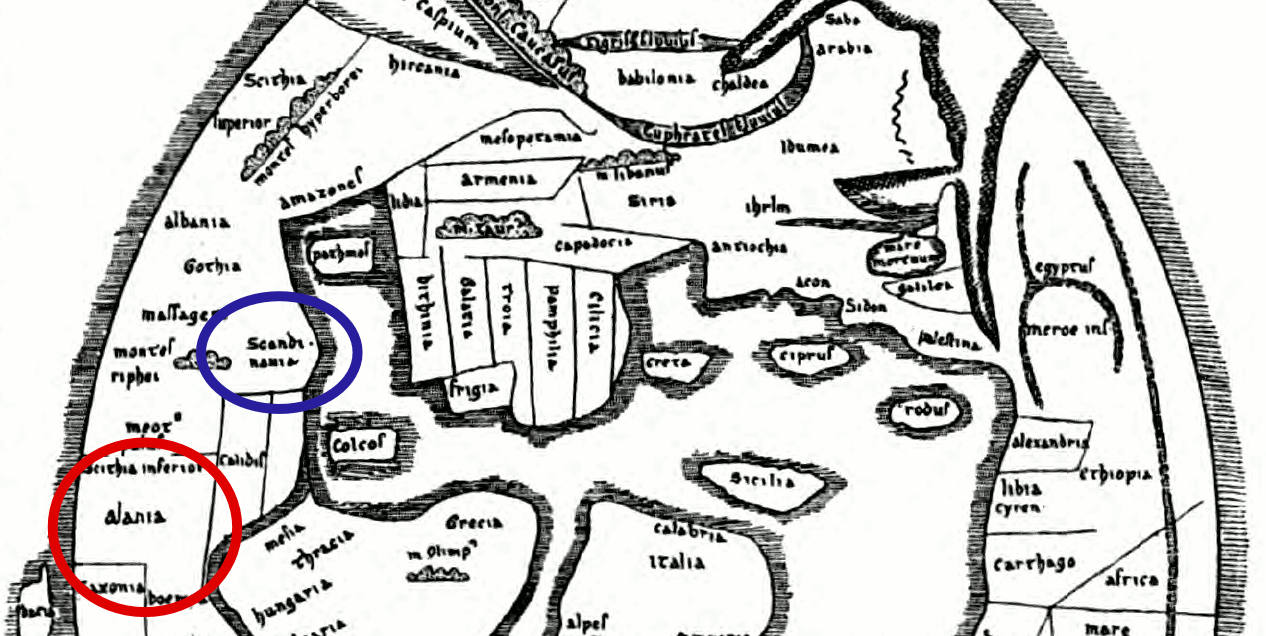
\includegraphics[width=\linewidth]{chast-colebanie-osnov/okartah/scand-01.jpg}
\end{center}

Ориентация примерно на восток. Я отметил цветными кружками Аланию (во Внутренней Скифии, Скитии) и Скандинавию. На береговом протяжении между ними – Мэот Палус, ныне Азовское море. Западнее (ниже) Скандинавии, в море – остров Колкос (Colcos), показанный на многих старинных картах и по названию имеющий отношение к Колхиде. Река возле Колкоса, исходя из лежащих у берегов ее стран – Дунай. Напротив Скандинавии, правее – полуостров Малой Азии. Восточнее, выше – Каспийское море (mare Caspium). К западу от Алании – Саксония. Запомним, это важно. Алания же – нынешняя Украина с Польшей.

Я бы отнес сию восточную Скандинавию к разряду диковинных ошибок и прошел мимо, если бы эта «ошибка» не была постоянной составляющей именно на картах к «Полихроникону». Давайте поглядим на другой вариант:

\begin{center}
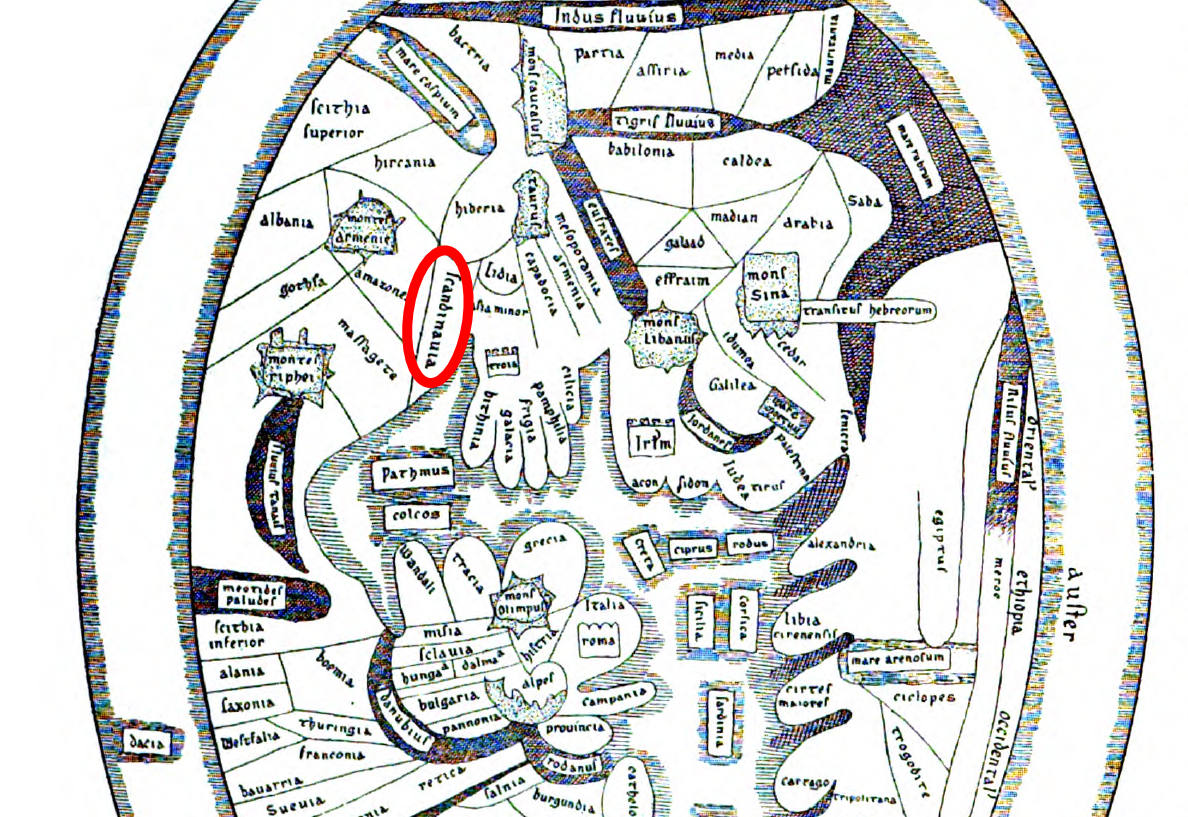
\includegraphics[width=\linewidth]{chast-colebanie-osnov/okartah/scand-02.jpg}
\end{center}

Скандинавия занимает здесь почти прежнее место у берега Черного моря, чуть сдвинувшись на восток (вверх), остальные границы прежние – Иберия, Амазонки, Мессагеты. Хорошо нарисован Танаис к западу от Скандинавии, а еще западнее – Мэотийское болото. Из карты следует, что Скандинавия находится на восток от Дона, однако выше Малой Азии. Это Кавказ либо Ставропольский край.

На современной карте Грузии, в тридцати километрах на восток от Кутаиси с трудом отыскивается село Сканде (სკანდე)\footnote{42°15'36"N 43°3'11"E}. Чуть севернее его – остатки крепости\footnote{42°16'6"N 43°2'46"E}. Это всё, что осталось от древних города и крепости Сканды (სკანდის ციხე, სკანდა).

На протяжении, быть может, тысячелетий она то разрушалась, то возрождалась, переходила из рук в руки, о ней забывали и вспоминали. Прокопий Кесарийский в «Войне с Персами» пишет, что в Лазике (западная Грузия) обжит лишь северный берег реки Риони, и:

\begin{quotation}
Все селения Лазов находятся здесь, на этой стороне реки, и тут издревле построены ими городки, в том числе самый укрепленный из них Археополь, Севастополь и крепость Питиунт, а у самых границ Ивиров Сканда и Сарапанис.
\end{quotation}

В обозримом по источникам прошлом Скандой владели то Греки, то Персы (Иранцы). Ее разрушил в 14 веке Тамерлан, но уже спустя несколько веков она служила пристанищем грузинской царице Тамаре, захватывалась попеременно то картлийскими, то имертинскими царями. Многократно о Сканде пишет грузинский историк 18 века Вахушти Багратиони в «Истории царства Грузинского».

А вот почитаем выдержку из «Статейного списка посольства в Имеретию 1650-1652 гг., составленного Алексеем Иевлевым»:

\begin{quotation}
И провожали послов до подворей азнауры. А что за столом цари подавали изперед себя послам кушенье, и те ествы прислали цари за послами к Микифору и Олексею на стан. А стоял Александр цар. под городом под Скандою, от города с полверсты; двор его учинен на площеди, на ровном месте поставлены поземные дощатые чердаки.

А город Сканда стоит на горе; каменой, четвероуголен, высок, сажен в десять. По стенам четыре башни а на башнех три пушечки волконейки, небольшие.

Да в городе ж церковь камена, без креста, во имя страстотерпца Георгия; в церкве стенное писмо. Да в церкве ж три образа: всемилостивого Спаса, да пречистые Богородицы, да Георгия страстотерпца; обложены серебром в чекан, позолочены; у спасова образа венец золот, писан мусиею. Да на городовой стене сделана полата болшая на трех житьях; а в верхнем житье лежит царева казна, и что прислано к нему Александру царю от ц-ого в-ва жалованье соболи, и те соболи положены в той же полате. И стерегут того города и казны тюфенчеи. Да в городе ж онбар болшой, деревяной насыпан полон хлеба; да вместо погреба вкопана в землю корчага болшая и налита виноградом на целой год, для осадного времени. А мерою того города около сто двадцать сажен болших.

Да около ж того города обрублено тарасы и насыпано хрящем. А всход к городу один и тот круг; взять приступом никоторыми мерами нельзя, гора каменная, да около обрубу, на той же горе, жилых дворов с тридцать. А иные дворы стоят под горами в стрелбище, и в два, и в полуверсте, и в версте, и боши, врозни, по крепким местом, для приходу воинских людей.

А от столного города Кутатиса до того города до Сканды верст с тридцать. А место пришло низ, ровнедь с долинами, верст на шестьдесят; а поперег от Сканда города до реки до Курлы верст с двадцать и болши. А места жилые, городки, и села, и деревни, и стоят по крепким местом, по речкам. И на том ровном месте многие царевы дворы устроены. А по другую сторону того ровного места, под гурелскими горами, течет река Курла. А течет из гурельские земли промеж гор, и вышла из гор в Олександрову землю, и впала в Реонь реку, от Кутатиса вест с шесть или с сем.
\end{quotation}

Когда крепость опустела – неведомо, равно как её создатели и время постройки. Туристы в Сканду не ходят, а краеведы туда добираются с трудом. Зная про Сканду, думаешь – так ли нелепа Скандинавия на старинных картах? Не являются ли они отголоском времени, когда крепость эта была, возможно, основой одноименной державы?

Что до нынешней Скандинавии, то ее часть в давнее время предстает в источниках то как единый остров Скандия, то несколькими островами, и постепенно обретает новое имя – Скандинавия. Под именем Scandia ее упоминает Птолемей в своей «Географии», для него это три острова: Нериг (давнее самоназвание Норвегии – Нориг), Берги и Думна. 

Сейчас Скандинавия известна как полуостров – но при повышенном уровне воды в океане могла быть цепью островов. С подписью «Скандии» полуостров изображается уже на картах 16 века, например на подробнейшей шведской морской карте Олафа Магнуса за 1530 год.

Языческие боги этой, привычной нам Скандинавии – Асы или Осы во главе с Одином – родом из Азии. Считается, потому и Асы, что от слова «Асия». В преданиях, Асы изначально предстают не богами, но могущественным сообществом людей, вроде Туаха Дэ Дананн. Обожествили их позже. \'Один же был, в некоторое время, просто предводителем Асов, колдуном и провидцем.

По «Саге Инглингов» (Ynglinga saga) из «Круга Земного» Снорри Стурлусона, Асы обитали в стране Асаланд или Асахэйм (Ásaland eða Ásaheimr), что лежит к востоку от реки Танаис, прежде именуемой Танаквисл или Ванаквисл (Tanakvísl eða Vanakvísl), впадающей в Черное море (Svartahafi). Страну в низовье этой реки называли Ваналанд или Ванахэйм, а ее жителей – Ванами. Главный же город в стране Асов – Асгард (Ásgarð). Ваны и Асы поначалу воевали, а после породнились. Ваны научили Асов своему колдовству.

Казалось бы, ясно сказано «Танаис». Но река Дон, с которой отождествляют Танаис, впадает в Азовское, а не Черное мое. Быть может, Снорри подразумевал под Танаисом другую реку, например Истр, Дунай? Но будем пока руководствоваться общепринятым толкованием, что Танаис это Дон.

По одним представлениям древних, Азия отделялась от Европы рекой Танаис. По другим представлениям, Азия – южное побережье Черного моря, известное в некоторые времена как Малая Азия.

В прологе «Младшей Эдды» сказано, что в Азии был город Троя, которой правил Тор, сын Меннона и Троан, дочери царя Приама. Из рода Тора происходил Один. В «Младшей Эдде» Троя отождествляется с Асгардом и помещена в Тыркланд (Tyrkland). А вроде бы известно, что сейчас это Турция. 

Малая Азия – часть Турции. Развалины Трои в ней показывают туристам. Впрочем нигде, кроме некоторых саг, Асгард не сопоставляется с Троей, а по географическому описанию из «Саги Инглингов», как увидим далее, Асгард находится эдак на Кавказе или в Ставропольи. 

В старину вообще многим народам было лестно ставить Троянцев себе в предки. И к сообщениям о сторонах света следует, наверное, тоже относиться  осторожно, памятуя о возможном смещении полюсов.

Я неоднократно сталкивался с тем, что в сагах одним словом именуют разные места. А ежели Тыркланд – это не Турция, а некие земли проживания народа Торков, что кочевал от Каспия до Винницы, Донбасса и Поросья? В самом деле, выходит, к востоку от Дона.

Стурлусон уточняет – Тыркланд лежит к югу от большого горного хребта, что тянется с северо-востока на юго-запад и отделяет Большую Свитьод (Svíþjóð ena Miklu) от других стран. Таким хребтом может быть Урал. Словом Svíþjóð в давних северных языках называли Швецию, а вот Большую Svíþjóð можно сопоставить со Большой Скифией, летописной «Великой Скуфью». Иногда впрочем вместо Большой Свитьод писали просто Свитьод, тогда надо было догадываться по смыслу, о чем идет речь.

Если определять положение Асгарда по «Младшей Эдде» и «Саге Инглингов», полагая Дон Танаисом, то выходит, что Асгард лежал к западу от Дона и южнее Урала. Это же Кавказ и Ставропольский край!

В «Саге Инглингов», Асы из Асгарда идут сперва на запад в Гардарики (Garðaríki, их соотносят с землями Киевской Руси), а затем отправляются на юг в Саксланд. В прологе «Младшей Эдды» про Гардарики ничего не сказано, но после странствий Один и его соратники попадают «на север» в Саксланд. Саксланд это будто север нынешней Германии, Саксония.

Выходит путаница, коль руководствоваться современными знаниями, положением полюса и считать сведения из саги истинными. Однако Саксланд лежит южнее Гардарики в случае, если полюс находится примерно там же, где у Птолемея, и привычную нам карту надо повернуть против часовой стрелки. Лишь тогда можно сказать, что Саксланд – южнее Гардарики.

Припомним карту из «Полихроникона» – Алания лежит рядом с Саксонией. Догадайтесь, что общего между Гардарики и большой Аланией от Бэкона, Хиджена, Исидора? То же, что у Киевской Руси да Роксолании – местность.

%Как бы ни было, родина Асов, по сагам, близка к Черному морю и обозначенному на старинных картах месту Скандинавии! Таким образом азиатская Скандинавия обретает весомую привязку. Значит, следует различать позднейшую «северную» Скандинавию с ранней азиатской. 

А теперь перекинем мостик от северной Скандинавии к восточной. В 50 километрах к западу от крепости Сканды лежит Южная Осетия. Грузины называют Осетинов – Оси. 

Север, Скандинавия, Асы. Восток, Скандинавия, Осы. Они же Асы, Ассы, Аланы.

Веками ученые пытались отыскать корни Осетинов, находя их то в Половцах, то в германских народах, то в семитских, пока в 19 веке не пришли к иранскому происхождению Осетинов, что немудрено по их самоназванию – Ирон, Ир! Но для такого очевидного вывода науке понадобились исследования академика Андрея Шегрена.

А ведь даже глядя на современную карту можно сразу сказать, что Осетия с Ираном – соседи. Вероятно, Осетины – потомки древних Иранцев, Персов, волей времени отмежеванные от большей части бывшей родины, которая простиралась до Осетии во времена царя Кира Великого, а затем Дария Первого. Государство Иран – ближайший по языку и месту жительства сосед Осетии!

Но благодаря работам Миллера и Абаева, наука считает теперь Осетинов потомками Аланов, Аланов потомками Сарматов, Сарматов потомками Скифов. Таким образом Абаев развил обоснование тому, что по иранскому в основе современного языка Осетинов можно достучаться до иранской же основы сарматского и скифского языков.

\begin{center}
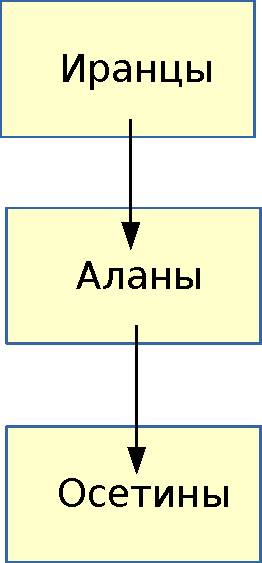
\includegraphics[width=0.20\linewidth]{chast-colebanie-osnov/okartah/iron02.pdf}

\textit{Схема примерного происхождения Осетинов по Абаеву.}
\end{center}

«Аланами» на этой схеме я для краткости обозначил цепочку Аланы – Сарматы – Скифы, а «Иранцами» именую жителей Ирана, ибо наука не объясняет, каким образом Скифам передался их язык. Приходится предполагать, подыгрывая науке, что от Иранцев.

В самом деле, Осетины живут ныне там, где раньше обитали Аланы – впрочем Аланы были и в нынешней Чечне, и около Днепра и во Франции да Италии, где поныне остались городки Аллейн, Алагна, Сармато Аландриано (Ландриано), Аллегно, Алано ди Пиаве. Славяне-Вандалы купно с Аланами обитали также в Испании, Галии, да по всей даже той части Европы, которую не считают славянской.

Поскольку Осетины называют себя Ирон, думаю, что народ из Ирана растворил в себе аланское население (не важно, коренное или пришлое), и потомки обоих народов и составляют нынешних Осетинов. Вместо того, чтобы предположить оба народа в «одновременные» предки Осетинов, Абаев сделал эти народы последовательными звеньями цепи происхождения.

Выражу взаимосвязь Иранцев, Аланов и Осетинов так:

\begin{center}
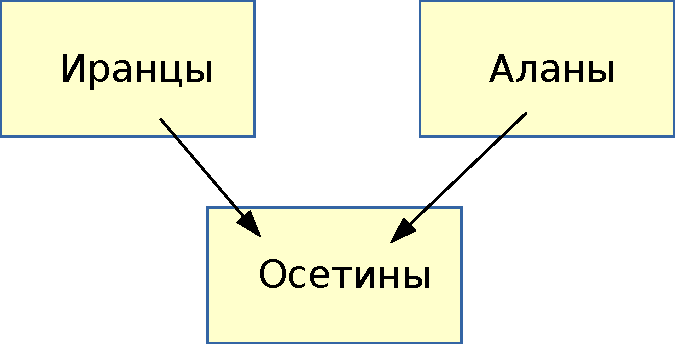
\includegraphics[width=0.50\linewidth]{chast-colebanie-osnov/okartah/iron01.pdf}
\end{center}

Влияние Иранцев оказалось сильнее, что выражается в языке и самоназвании – Ирон.

В обозримом прошлом, в осетинском языке не было слова «Алан», пока его не заимствовали из общекультурной среды. А то, что Аланы – давнее самоназвание Ирон, Абаев вывел следующим образом.
 
В преданиях Осетинов существует загадочное выражение «аллон-биллон»\footnote{Кстати, в чеченской сказке «Черкес Иса и чеченец Иса» упомянуто чудесное существо по имени Алла-Белла, обитавшее в пещере.}. Подобно тому, как в русских сказках Баба Яга принюхивается и подозревает, что здесь пахнет русским духом, так в осетинских людоед-великан отмечает – мол, пахнет аллон-биллоном! Абаев не смог истолковать «биллон», однако «аллон» сопоставил с человеком, который находился рядом с великаном. Значит, человек тот – непременно Алан – решил Абаев. А следовательно, предок Осетинов.

О ком же речь идет в преданиях с «аллон-биллон»? Кого вынюхивал людоед? Он вынюхивал Нартов. 

Нарты – народ, о котором рассказывают Осетины в своих преданиях. Нарты сгинули, их покарал бог за дерзость. Ученые гутарят, что в нартовском эпосе отразились Скифы, а Нарты – предки Осетинов. Но ведь сами Осетины говорят – Нарты все погибли. 

К сожалению, еще мало преданий о Нартах переведено на другие языки. А ведь это культурный пласт, сопоставимый по размаху с греческой и северной мифологией, и в некоторых подробностях удивительно перекликающийся с ирландской.

Связь с Ирландией проявляется во многом.

Ирландия, или, в старину – Ир-лонд, земля Иров\footnote{Произношение «Айрлэнд» – английское, на современном ирландском языке звучание иное – «эйжэ», а как оно звучало в старину, неизвестно, есть давнее написание Ériu. В преданиях так звали дочь Эрнмаса из числа Туаха Дэ Дананн. Другой вариант имени – Эрин, почти как Ирина.}. А как называют себя Осетины? Ирами.

Среди Осетинов и Ирландцев рыжих людей больше, чем среди других народов.

Далее. Когда я еще думал, что все Аланы были ираноязычны, то решил, что Туаха Дэ Дананн (Tuatha Dé Danann) можно перевести просто – народы богини Реки, толкуя «Дану» как производное от иранского корня «дон» или «дан».

Правда, в Ирландии не знали богиню Дану. Слово «Дану» вообще придумано учеными, они сочли, что «Danann» это склоненное в притяжательном падеже имя Danu. Мол, чьи народы? Danann. Tuath(а) значит народ(ы), De – божество.% Вместе произносится как «туаха дэ данан», где «дэ» размытое, в нем слышится «ч». 

А если «дэ даннан» – подражание другим словам либо искаженная их передача? В преданиях Осетинов о Нартах важнейшую роль играет чародейка, воительница и советчица по имени Сат\'ана. Я сам не люблю игру с буквами, но «дэдананн» c заменой второй «д» на «т» может звучать как «тэтананн» или «сэтананн».

Сатана – богиня или полубогиня, росшая не по дням, а по часам – за месяц как за год. Это свойство, в преданиях, присуще тем, в ком течет нечеловеческая кровь. Сатана умеет принимать множество образов – являться старухой или молодой\footnote{В 13 веке шотландец Томас Лермонт (Thomas Learmonth the Rhymer) по прозвищу Рифмач (возможно, Михаил Лермонтов – из его рода), провидец, побывал в мире Эльфов, Элфхэйме. Тамошняя королева Фэйри обладала способностью менять свой возраст с молодого на старческий. Три дня прожил Лермонт среди чудесного народа, семь лет прошло в нашем мире. Пробыв некоторое время с людьми, он вернулся в Элфхэйм. Общение с народом Фэйри и королевой Фэйри хорошо освещено в документах из шотландских, 15-18 веков, судилищ над ведьмами. За такое общение, действительное или мнимое, людям со стороны людей же грозили пытки и сожжение заживо. Скиф Анахарсис на вопрос, что самое опасное для человека, отвечал – сам человек.}, понимает птичий язык, управляет погодой, о событиях в мире знает, глядя в некое «небесное зеркало». В сказаниях Сатану описывают как «неба коварство, земли колдовство». 

%По Геродоту, родоначальником скифов был некий Таргитаос: «Родители его были, как говорят, Зевс и дочь реки Борисфен». А в нартовском эпосе, Сатана – дочь Уастырджи

Возможно, Туаха Дэ Дананн следует толковать как «народ Сат\'аны»?

Героические предания Осетинов порой сходны с ирландскими. Часто сравнивают повествования о Сослане (Осетия) и Кухулине (Ирландия). Среди общих подробностей: у Сослана в каждом глазу по два зрачка, у Кухулина четыре в одном, три в другом. Кухулин гибнет потому, что его колесницу зачаровала отвергнутая им богиня войны, призрачная королева Морриган. Отвергнутая богиня же посылает на Сослана самоходную повозку Колесо Ойнона (Балсага, Малсага, Барсага). 

Серебряная рука короля из Анналов Ирландии – и осетинский богатырь Сослан, с телом из черного булата и железными ногами, а также металлический Батраз, столь могущественный, что вступил в распрю с жителями неба и был убит богом при помощи Колеса Балсага. По другому варианту, его расстреляли Елиаты, подлетев в облаке, которое рассеивалось, когда Батраз стрелял в ответ. Батраз раскалился и упал, и ему нечем было охладиться. Он долго лежал. Никто не мог приближаться, умирали, даже противники, жители неба – Зэды и Дуаги.

Не от Нартов ли пошли Туаха Дэ Дананн и обожествленные Асы? Кто такие Нарты в представлении Осетинов? Откроем второй том трехтомника «Нарты»\cite{narty01}. Про народы былых времен сказано:

\begin{quotation}
1. О гумирах\\

Гумиры были огромными, сильными, но глупыми людьми. Они не понимали, что от огня можно отодвинуться, и прикрывали себе лица [кусками] сланца или дерева. Однажды они увидели, как собака все дальше отползала от костра по мере того, как он разгорался. Так гумиры научились оберегать себя от огня.\\

2. Нарты\\

До нартов [на земле] жили гумиры, топоров у них не было, деревья они вырывали руками. Потом появились уаиги – крупные, могучие люди. Вслед за ними [появился] нартовский народ.

Сотворив мир, бог решил создать людей. По его велению на земле появились уадмиры. Были это люди огромные и сильные, в ущельях они не помещались, земле их было трудно выдержать.

Триста лет прошло, и сотворил бог вслед за уадмирами камбада – умом и силой на уадмиров похожие, а ростом невысокие, не выше нынешних десятилетних детей. Слишком малыми оказались камбада для жизни на земле\footnote{Что впрочем, не мешало им жить дальше, судя по сказаниям. Так, герой нартовских сказаний Сослан встречает низенького, очень сильного охотника, и тот называет себя камбада.}.

Триста лет прошло, и сотворил бог вслед за камбада гамеров, но и они оказались слишком велики и ростом и силой.

И еще триста лет прошло, и сотворил бог вслед за гамерами гумиров. Не вышли и они под стать земле. Триста лет прошло, и сотворил бог вслед за гумирами уаигов. Не удались и они, слишком крупными оказались. Триста лет прошло, и сотворил бог вслед за уаигами новый народ, нартов, и удались они ему, ростом и силой были под стать земле. [...] \\

5. Происхождение нартов\\

До нартов на свете жили уадмеры. Уадмеры были огромными людьми, дома не строили: «Если мы будем наклонять головы, проходя через порог [в двери], то бог подумает, что мы ему кланяемся». Бог очень скоро их уничтожил. После этого появились уаиги – грубые, сильные, безобразные: у кого было семь голов, у кого – одна голова и один глаз\footnote{Сходство с Фомойри и Песиголовцами.}. Жили они в горах, лесах и пещерах. Когда появились нарты, то они сражались с уаигами и уничтожили их\footnote{Туаха Дэ Дананн тоже сражались с Фомойри.}. Откуда появились нарты, этого, кроме бога, никто не знает, но в сказаниях говорят, что они появились со дна моря.
\end{quotation}

Нарты легко роднятся с подводными жителями Донбеттырами, носят латы, вооружены мечами, ружьями и пистолетами, а когда им нужно рассмотреть что-то далекое, смотрят в подзорные трубы. В подзорные трубы смотрят и русские богатыри в тех былинах, которых не коснулась рука великомудрых редакторов, после чего богатыри глядят уже не в оптические приборы, но из-под ладони или в кулак. Хлебом нартам служит кукуруза.

Нарты – не боги, однако приглашают на свои пиры богов. Их перечисляют в предании о Сослане, и боги представлены как обычные действующие лица:

\begin{quotation} 
Были званы на пир также небесные зэды и дауаги; покровитель путников бесстрашный Уастырджи\footnote{Отец Сатаны, может летать, надевая золотые крылья. Летали также мелеки – обитатели неба. А подземные жители, что похищали людей в свои пещеры, именовались бценагами.}, небесный Курдагалон, покровители скота Тутыр и Афсати, покровитель зерца Уацилла, светлый Реком и чистый Мыкалгабырта, небесный Сафа\footnote{Бог оружия, создатель знаменитых мечей.} и Галагон, а также покровитель вод Донбеттыр.
\end{quotation} 

Нарты тоже не просты, они могут перемещаться в летающих башнях, как например Бедуха из Ахсартаггата в предании о Сослане. Нарты  пользуются и меньшими средствами передвижения – самоходными повозками (хадтулга уардон).

И когда речь идет об огнестрельном оружии, почему мы должны полагать, что оно было введено в предание сравнительно недавно? Думаю, оно было там издревле. И вещи названы своими именами, без опрощения вроде грома и молний.

В преданиях не определяется родственность Осетинов к Нартам. Предшествующее население Осетии? Народ, который соприкоснулся с Ирон и Аланами, затем сгинул, но оставил о себе память в преданиях?
 
Считалось, что Нарты не подчинялись богам – ни разным покровителям, ни главному. Даже дверные косяки делали высокими, чтобы не наклоняться, дабы бог не подумал, что это в его честь. Отношения между Нартами, богом и жителями неба накалились до предела, Батраз вступил в открытое противостояние с последними и был повержен. Следует расправа над остальными Нартами.

По одному из преданий, когда бог покончил с Батразом, Нарты бросили меч того в воду, отчего пошли «волны и ураганы», а море закипело и приобрело красный цвет. Затем бог уничтожил Нартов огнем с небес. В другом предании Нарты умирают от голода, после неурожая. В третьем – бог обрушивает на них гору. В еще одном сказании Нарты выкапывают себе могилы и бросаются туда. Это полностью совпадает с некоторыми из преданий об исходе странного народа Чуди белоглазой.

Потомки восточных Аланов донесли до нас предания о своем далеком прошлом. У потомков Аланов западных таких преданий не осталось.
